\documentclass{fkssolpub}

\usepackage[czech]{babel}
\usepackage{fontspec}
\usepackage{fkssugar}
\usepackage{amsmath}
\usepackage{graphicx}

\author{Ondřej Sedláček}
\school{Gymnázium Oty Pavla} 
\series{1}
\problem{2} 

\begin{document}

\begin{figure}
	\begin{center}
		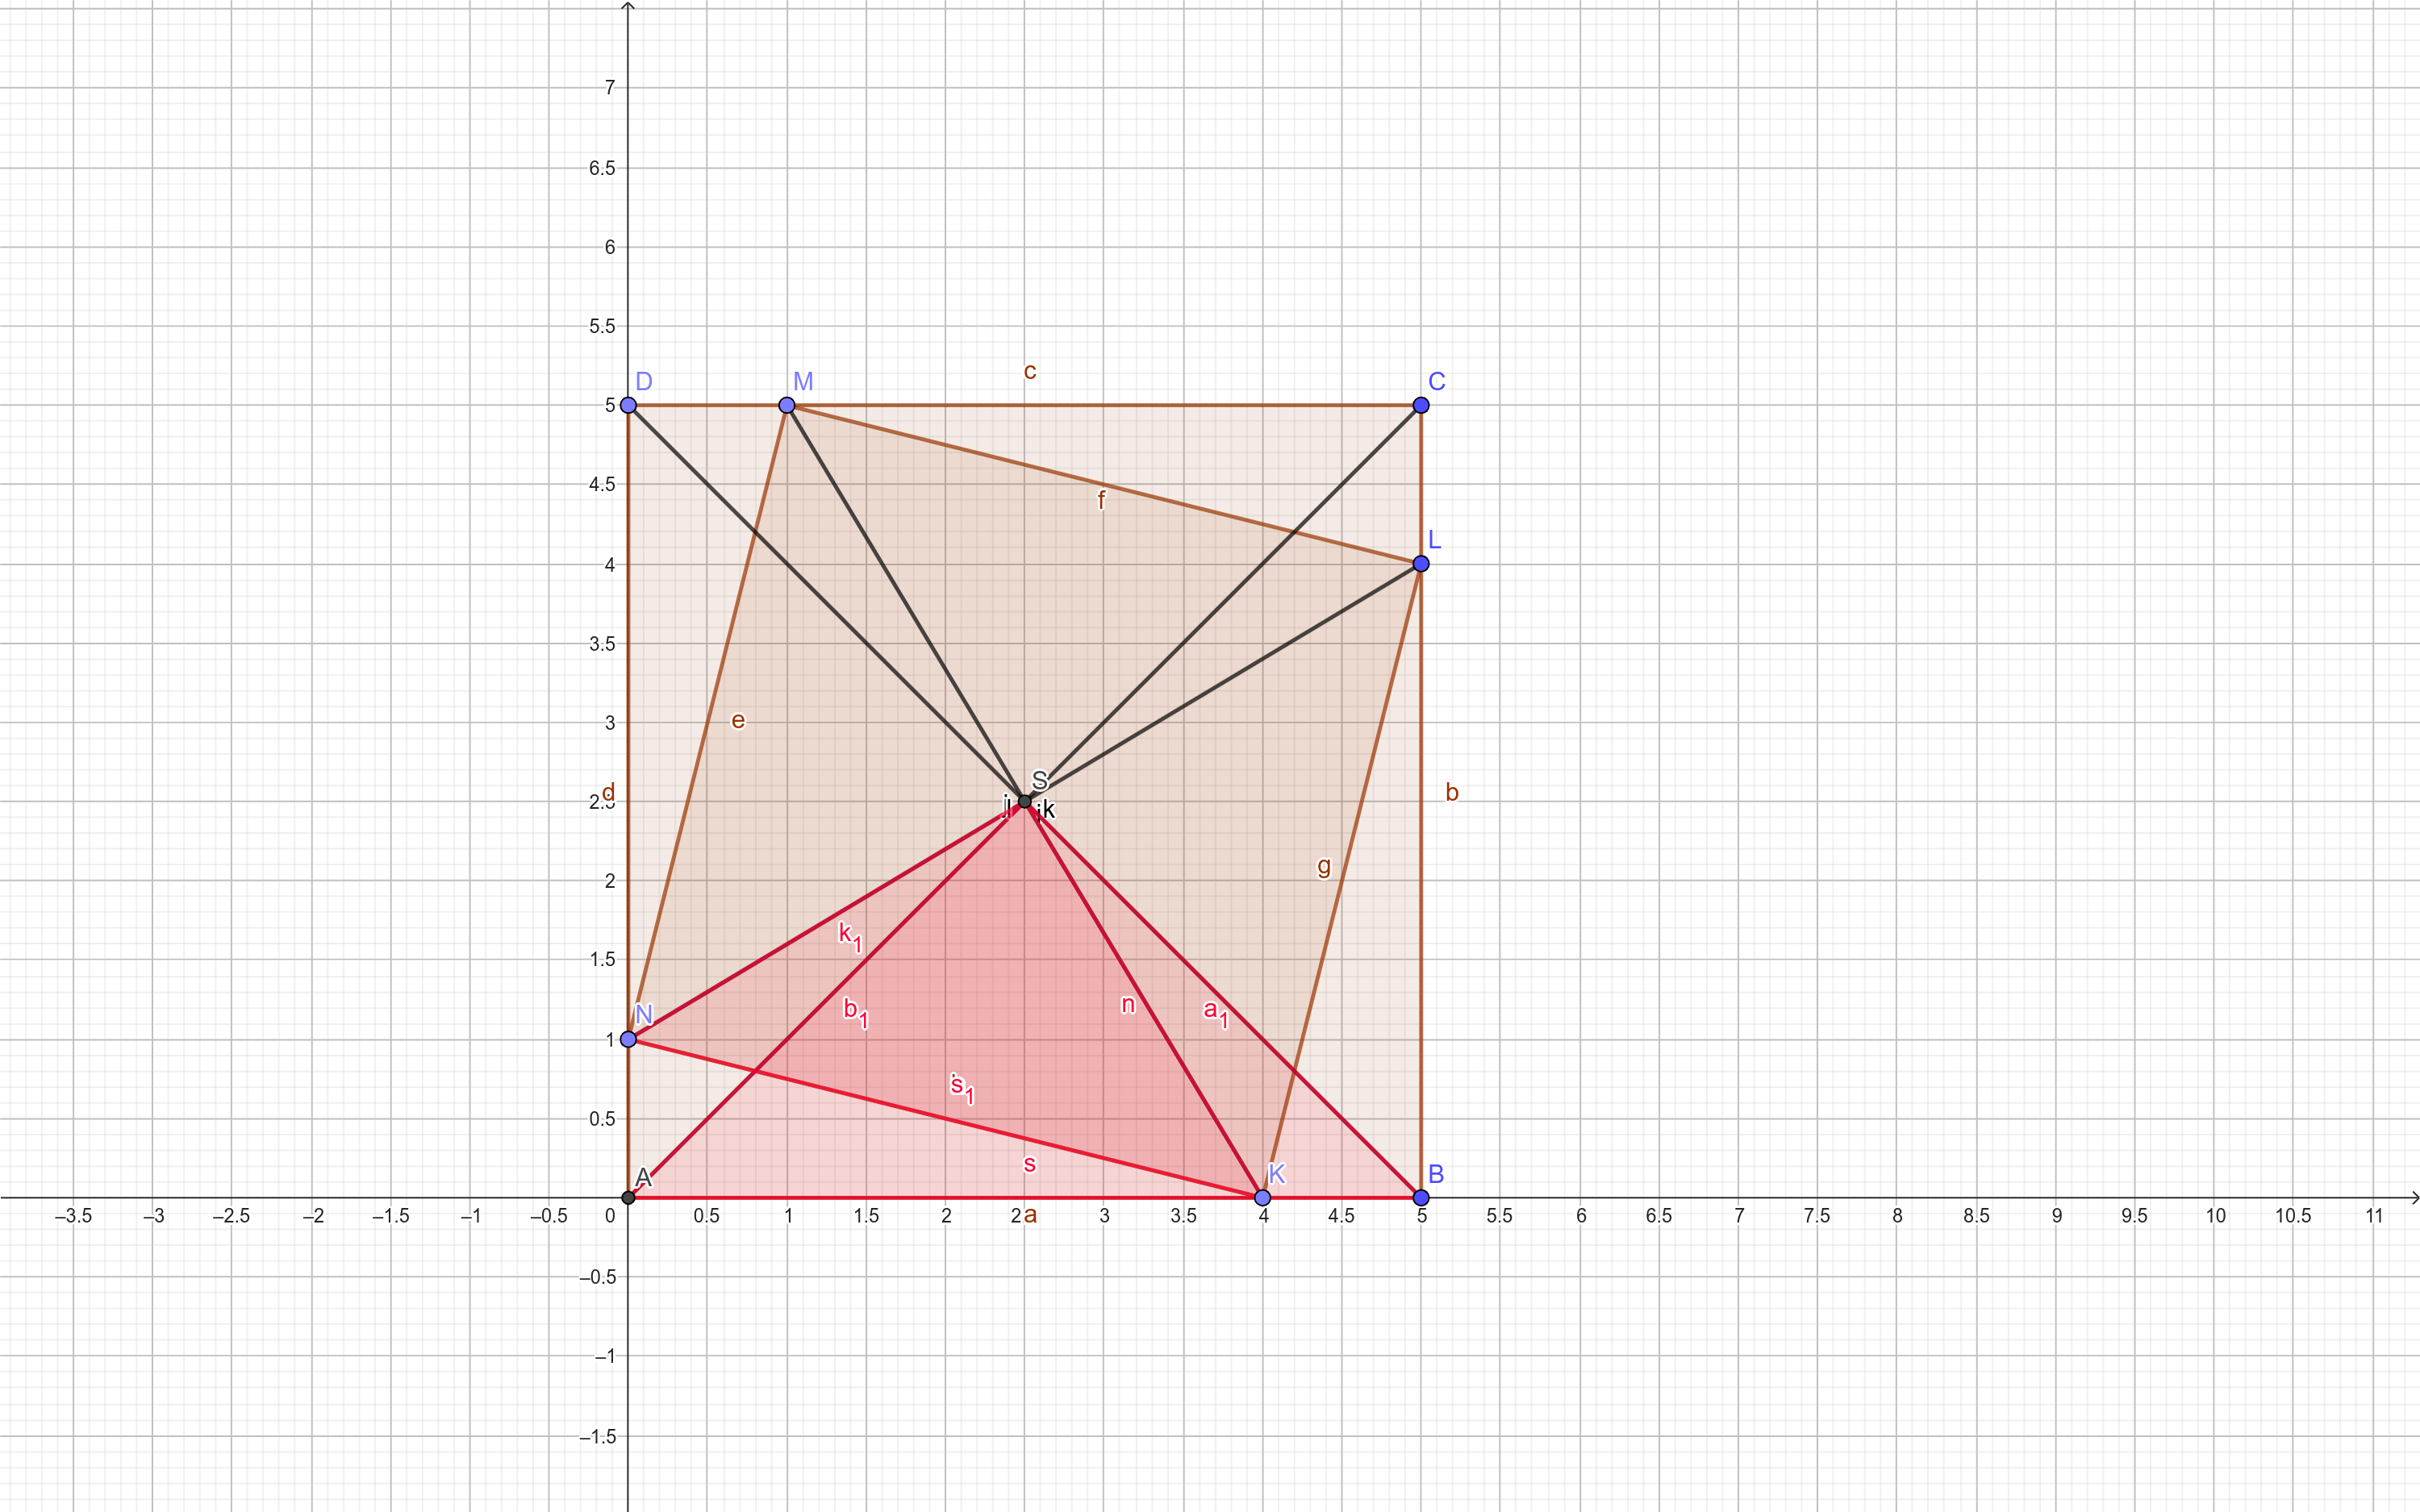
\includegraphics[width=0.95\textwidth]{2-fig}
	\end{center}
	\caption{Konstrukce úlohy}
	\label{fig:1}
\end{figure}

Jako první si všimneme toho, že trojúhelníky $AKN$ a $CML$ jsou shodné, stejně jako trojúhelníky $BLK$ a $DNM$, podle věty usu. Toho můžeme využít k tomu, abychom ukázali, že průsečíky úhlopříček obou obdélníku jsou ve stejném bodě $S$. Poněvadž víme, že $|AN| = |CL|$ a $AN \parallel CL$, pak podle věty usu jsou trojúhelníky $ASN$ a $CSL$ shodné, tím pádem $|AS| = |CS|$ a zároveň $|NS| = |LS|$, z čehož vyplývá to, že bod $S$ je střed obou obdélníků.

Teď už dokážeme, že $ABCD$ je čtverec. Pokud dokážeme, že $|AN| = |KB|$, pak protože jsou si trojúhelníky $BLK$ a $AKN$ podobné, dokážeme shodnost těchto trojúhelníků a tím pádem shodnost všech trojúhelníků $AKN$, $BLK$, $CML$ a $DNM$. Víme, že trojúhelníky $ASB$ a $NSK$ jsou si spirálně podobné, tím pádem $BSK$ a $ASN$ jsou si též spirálně podobné, a protože $|AS| = |BS|$, pak jsou si trojúhelníky $BSK$ a $ASN$ shodné a dokázali jsme tím rovnost $|AN| = |KB|$.

Tím jsme ukázali, že $ABCD$ je čtverec, čímž je důkaz u konce.

\end{document}
